% Options for packages loaded elsewhere
\PassOptionsToPackage{unicode}{hyperref}
\PassOptionsToPackage{hyphens}{url}
%
\documentclass[
]{article}
\usepackage{amsmath,amssymb}
\usepackage{lmodern}
\usepackage{ifxetex,ifluatex}
\ifnum 0\ifxetex 1\fi\ifluatex 1\fi=0 % if pdftex
  \usepackage[T1]{fontenc}
  \usepackage[utf8]{inputenc}
  \usepackage{textcomp} % provide euro and other symbols
\else % if luatex or xetex
  \usepackage{unicode-math}
  \defaultfontfeatures{Scale=MatchLowercase}
  \defaultfontfeatures[\rmfamily]{Ligatures=TeX,Scale=1}
\fi
% Use upquote if available, for straight quotes in verbatim environments
\IfFileExists{upquote.sty}{\usepackage{upquote}}{}
\IfFileExists{microtype.sty}{% use microtype if available
  \usepackage[]{microtype}
  \UseMicrotypeSet[protrusion]{basicmath} % disable protrusion for tt fonts
}{}
\makeatletter
\@ifundefined{KOMAClassName}{% if non-KOMA class
  \IfFileExists{parskip.sty}{%
    \usepackage{parskip}
  }{% else
    \setlength{\parindent}{0pt}
    \setlength{\parskip}{6pt plus 2pt minus 1pt}}
}{% if KOMA class
  \KOMAoptions{parskip=half}}
\makeatother
\usepackage{xcolor}
\IfFileExists{xurl.sty}{\usepackage{xurl}}{} % add URL line breaks if available
\IfFileExists{bookmark.sty}{\usepackage{bookmark}}{\usepackage{hyperref}}
\hypersetup{
  pdftitle={7\_Vis\_CCM\_Sig\_Causal\_Vars},
  pdfauthor={Kurt Ingeman},
  hidelinks,
  pdfcreator={LaTeX via pandoc}}
\urlstyle{same} % disable monospaced font for URLs
\usepackage[margin=1in]{geometry}
\usepackage{color}
\usepackage{fancyvrb}
\newcommand{\VerbBar}{|}
\newcommand{\VERB}{\Verb[commandchars=\\\{\}]}
\DefineVerbatimEnvironment{Highlighting}{Verbatim}{commandchars=\\\{\}}
% Add ',fontsize=\small' for more characters per line
\usepackage{framed}
\definecolor{shadecolor}{RGB}{248,248,248}
\newenvironment{Shaded}{\begin{snugshade}}{\end{snugshade}}
\newcommand{\AlertTok}[1]{\textcolor[rgb]{0.94,0.16,0.16}{#1}}
\newcommand{\AnnotationTok}[1]{\textcolor[rgb]{0.56,0.35,0.01}{\textbf{\textit{#1}}}}
\newcommand{\AttributeTok}[1]{\textcolor[rgb]{0.77,0.63,0.00}{#1}}
\newcommand{\BaseNTok}[1]{\textcolor[rgb]{0.00,0.00,0.81}{#1}}
\newcommand{\BuiltInTok}[1]{#1}
\newcommand{\CharTok}[1]{\textcolor[rgb]{0.31,0.60,0.02}{#1}}
\newcommand{\CommentTok}[1]{\textcolor[rgb]{0.56,0.35,0.01}{\textit{#1}}}
\newcommand{\CommentVarTok}[1]{\textcolor[rgb]{0.56,0.35,0.01}{\textbf{\textit{#1}}}}
\newcommand{\ConstantTok}[1]{\textcolor[rgb]{0.00,0.00,0.00}{#1}}
\newcommand{\ControlFlowTok}[1]{\textcolor[rgb]{0.13,0.29,0.53}{\textbf{#1}}}
\newcommand{\DataTypeTok}[1]{\textcolor[rgb]{0.13,0.29,0.53}{#1}}
\newcommand{\DecValTok}[1]{\textcolor[rgb]{0.00,0.00,0.81}{#1}}
\newcommand{\DocumentationTok}[1]{\textcolor[rgb]{0.56,0.35,0.01}{\textbf{\textit{#1}}}}
\newcommand{\ErrorTok}[1]{\textcolor[rgb]{0.64,0.00,0.00}{\textbf{#1}}}
\newcommand{\ExtensionTok}[1]{#1}
\newcommand{\FloatTok}[1]{\textcolor[rgb]{0.00,0.00,0.81}{#1}}
\newcommand{\FunctionTok}[1]{\textcolor[rgb]{0.00,0.00,0.00}{#1}}
\newcommand{\ImportTok}[1]{#1}
\newcommand{\InformationTok}[1]{\textcolor[rgb]{0.56,0.35,0.01}{\textbf{\textit{#1}}}}
\newcommand{\KeywordTok}[1]{\textcolor[rgb]{0.13,0.29,0.53}{\textbf{#1}}}
\newcommand{\NormalTok}[1]{#1}
\newcommand{\OperatorTok}[1]{\textcolor[rgb]{0.81,0.36,0.00}{\textbf{#1}}}
\newcommand{\OtherTok}[1]{\textcolor[rgb]{0.56,0.35,0.01}{#1}}
\newcommand{\PreprocessorTok}[1]{\textcolor[rgb]{0.56,0.35,0.01}{\textit{#1}}}
\newcommand{\RegionMarkerTok}[1]{#1}
\newcommand{\SpecialCharTok}[1]{\textcolor[rgb]{0.00,0.00,0.00}{#1}}
\newcommand{\SpecialStringTok}[1]{\textcolor[rgb]{0.31,0.60,0.02}{#1}}
\newcommand{\StringTok}[1]{\textcolor[rgb]{0.31,0.60,0.02}{#1}}
\newcommand{\VariableTok}[1]{\textcolor[rgb]{0.00,0.00,0.00}{#1}}
\newcommand{\VerbatimStringTok}[1]{\textcolor[rgb]{0.31,0.60,0.02}{#1}}
\newcommand{\WarningTok}[1]{\textcolor[rgb]{0.56,0.35,0.01}{\textbf{\textit{#1}}}}
\usepackage{graphicx}
\makeatletter
\def\maxwidth{\ifdim\Gin@nat@width>\linewidth\linewidth\else\Gin@nat@width\fi}
\def\maxheight{\ifdim\Gin@nat@height>\textheight\textheight\else\Gin@nat@height\fi}
\makeatother
% Scale images if necessary, so that they will not overflow the page
% margins by default, and it is still possible to overwrite the defaults
% using explicit options in \includegraphics[width, height, ...]{}
\setkeys{Gin}{width=\maxwidth,height=\maxheight,keepaspectratio}
% Set default figure placement to htbp
\makeatletter
\def\fps@figure{htbp}
\makeatother
\setlength{\emergencystretch}{3em} % prevent overfull lines
\providecommand{\tightlist}{%
  \setlength{\itemsep}{0pt}\setlength{\parskip}{0pt}}
\setcounter{secnumdepth}{-\maxdimen} % remove section numbering
\ifluatex
  \usepackage{selnolig}  % disable illegal ligatures
\fi

\title{7\_Vis\_CCM\_Sig\_Causal\_Vars}
\author{Kurt Ingeman}
\date{6/27/2021}

\begin{document}
\maketitle

\begin{Shaded}
\begin{Highlighting}[]
\FunctionTok{rm}\NormalTok{(}\AttributeTok{list =} \FunctionTok{ls}\NormalTok{())}

\FunctionTok{library}\NormalTok{(here)}
\end{Highlighting}
\end{Shaded}

\begin{verbatim}
## here() starts at /Users/kurtingeman/github/CORE
\end{verbatim}

\begin{Shaded}
\begin{Highlighting}[]
\FunctionTok{library}\NormalTok{(tidyr)}
\FunctionTok{library}\NormalTok{(dplyr)}
\end{Highlighting}
\end{Shaded}

\begin{verbatim}
## 
## Attaching package: 'dplyr'
\end{verbatim}

\begin{verbatim}
## The following objects are masked from 'package:stats':
## 
##     filter, lag
\end{verbatim}

\begin{verbatim}
## The following objects are masked from 'package:base':
## 
##     intersect, setdiff, setequal, union
\end{verbatim}

\begin{Shaded}
\begin{Highlighting}[]
\FunctionTok{library}\NormalTok{(RColorBrewer)}
\FunctionTok{library}\NormalTok{(ggplot2)}
\end{Highlighting}
\end{Shaded}

\begin{Shaded}
\begin{Highlighting}[]
\NormalTok{df }\OtherTok{\textless{}{-}}  \FunctionTok{read.csv}\NormalTok{(}\FunctionTok{here}\NormalTok{(}\StringTok{"CORE EDM Visual"}\NormalTok{, }\StringTok{"CORE\_reduce\_CCM\_vars"}\NormalTok{, }\StringTok{"CCM\_twin\_95.csv"}\NormalTok{))}
\CommentTok{\# 250 vars}

\CommentTok{\# ensure that max will work when all values negative}
\CommentTok{\# df[is.na(df)] \textless{}{-} {-}99}

\CommentTok{\# split df into the rec4 and rec5 values}
\NormalTok{df4 }\OtherTok{\textless{}{-}}\NormalTok{ df }\SpecialCharTok{\%\textgreater{}\%} 
  \FunctionTok{select}\NormalTok{(}\DecValTok{1}\SpecialCharTok{:}\DecValTok{8}\NormalTok{) }\SpecialCharTok{\%\textgreater{}\%} 
  \FunctionTok{rename}\NormalTok{(}
    \AttributeTok{ESU =}\NormalTok{ ESU\_rec4n,}
    \AttributeTok{IMN =}\NormalTok{ Imnaha\_rec4n,}
    \AttributeTok{MFS =}\NormalTok{ Middle.Fork.Salmon\_rec4n, }
    \AttributeTok{UPS =}\NormalTok{ Upper.Salmon\_rec4n}
\NormalTok{  )}

\NormalTok{df5 }\OtherTok{\textless{}{-}}\NormalTok{ df }\SpecialCharTok{\%\textgreater{}\%} 
  \FunctionTok{select}\NormalTok{(}\DecValTok{1}\SpecialCharTok{:}\DecValTok{4}\NormalTok{, }\DecValTok{9}\SpecialCharTok{:}\DecValTok{12}\NormalTok{) }\SpecialCharTok{\%\textgreater{}\%} 
  \FunctionTok{rename}\NormalTok{(}
    \AttributeTok{ESU =}\NormalTok{ ESU\_rec5n,}
    \AttributeTok{IMN =}\NormalTok{ Imnaha\_rec5n,}
    \AttributeTok{MFS =}\NormalTok{ Middle.Fork.Salmon\_rec5n, }
    \AttributeTok{UPS =}\NormalTok{ Upper.Salmon\_rec5n}
\NormalTok{  )}
\end{Highlighting}
\end{Shaded}

\hypertarget{are-predators-drivers-of-salmon-recruitment}{%
\section{1. Are predators drivers of salmon
recruitment}\label{are-predators-drivers-of-salmon-recruitment}}

\hypertarget{evidence-exceed-ccm-thresholds-can-recover-causal-vars-from-salmon-dynamics}{%
\subsection{evidence: Exceed CCM thresholds, can recover causal vars
from salmon
dynamics}\label{evidence-exceed-ccm-thresholds-can-recover-causal-vars-from-salmon-dynamics}}

\hypertarget{rec4-visualize-the-distribution-of-urho-values-for-broadest-categories-of-causal-variables}{%
\subsection{Rec4: Visualize the distribution of uRho values for broadest
categories of causal
variables}\label{rec4-visualize-the-distribution-of-urho-values-for-broadest-categories-of-causal-variables}}

\hypertarget{create-new-variables-to-distiguish-oceanographic-biological-and-human-variables}{%
\subsubsection{Create new variables to distiguish oceanographic,
biological, and human
variables}\label{create-new-variables-to-distiguish-oceanographic-biological-and-human-variables}}

\begin{Shaded}
\begin{Highlighting}[]
\NormalTok{df }\OtherTok{\textless{}{-}}\NormalTok{ df }\SpecialCharTok{\%\textgreater{}\%} 
  \FunctionTok{filter}\NormalTok{(}\SpecialCharTok{!}\NormalTok{cat }\SpecialCharTok{==} \StringTok{"flow"}\NormalTok{) }\SpecialCharTok{\%\textgreater{}\%} 
  \FunctionTok{filter}\NormalTok{(}\SpecialCharTok{!}\NormalTok{cat }\SpecialCharTok{==} \StringTok{"hseal"}\NormalTok{) }\SpecialCharTok{\%\textgreater{}\%} 
  \FunctionTok{mutate}\NormalTok{(}\AttributeTok{domain =} \FunctionTok{case\_when}\NormalTok{(}
\NormalTok{    cat }\SpecialCharTok{==} \StringTok{"arc"} \SpecialCharTok{|}\NormalTok{ cat }\SpecialCharTok{==} \StringTok{"pdo"} \SpecialCharTok{|}\NormalTok{ cat }\SpecialCharTok{==} \StringTok{"upw"} \SpecialCharTok{|}\NormalTok{ cat }\SpecialCharTok{==} \StringTok{"npgo"} \SpecialCharTok{\textasciitilde{}} \StringTok{"ocean"}\NormalTok{, }
\NormalTok{    cat }\SpecialCharTok{==} \StringTok{"ssl"} \SpecialCharTok{|}\NormalTok{ cat }\SpecialCharTok{==} \StringTok{"csl"} \SpecialCharTok{|}\NormalTok{ cat }\SpecialCharTok{==} \StringTok{"orca"} \SpecialCharTok{|}\NormalTok{ cat }\SpecialCharTok{==} \StringTok{"hseal"} \SpecialCharTok{\textasciitilde{}} \StringTok{"predator"}\NormalTok{, }
\NormalTok{    cat }\SpecialCharTok{==} \StringTok{"harv"} \SpecialCharTok{|}\NormalTok{ cat }\SpecialCharTok{==} \StringTok{"hatch"} \SpecialCharTok{\textasciitilde{}} \StringTok{"human"}\NormalTok{)) }\SpecialCharTok{\%\textgreater{}\%} 
  \FunctionTok{group\_by}\NormalTok{(domain) }\SpecialCharTok{\%\textgreater{}\%} 
  \FunctionTok{mutate}\NormalTok{(}\AttributeTok{mu\_ESU =} \FunctionTok{mean}\NormalTok{(ESU\_rec4n, }\AttributeTok{na.rm=}\ConstantTok{TRUE}\NormalTok{)) }\SpecialCharTok{\%\textgreater{}\%}
  \FunctionTok{ungroup}\NormalTok{()}
\end{Highlighting}
\end{Shaded}

\hypertarget{histogram-of-distribution-of-urho-values-facet-by-domain}{%
\subsubsection{Histogram of distribution of uRho values, facet by
domain}\label{histogram-of-distribution-of-urho-values-facet-by-domain}}

\begin{Shaded}
\begin{Highlighting}[]
\FunctionTok{ggplot}\NormalTok{(df, }\FunctionTok{aes}\NormalTok{(}\AttributeTok{x=}\NormalTok{ESU\_rec4n)) }\SpecialCharTok{+} \FunctionTok{geom\_histogram}\NormalTok{(}\AttributeTok{color=}\StringTok{"black"}\NormalTok{, }\AttributeTok{fill=}\StringTok{"white"}\NormalTok{, }\AttributeTok{binwidth=}\FloatTok{0.01}\NormalTok{)}
\end{Highlighting}
\end{Shaded}

\begin{verbatim}
## Warning: Removed 22 rows containing non-finite values (stat_bin).
\end{verbatim}

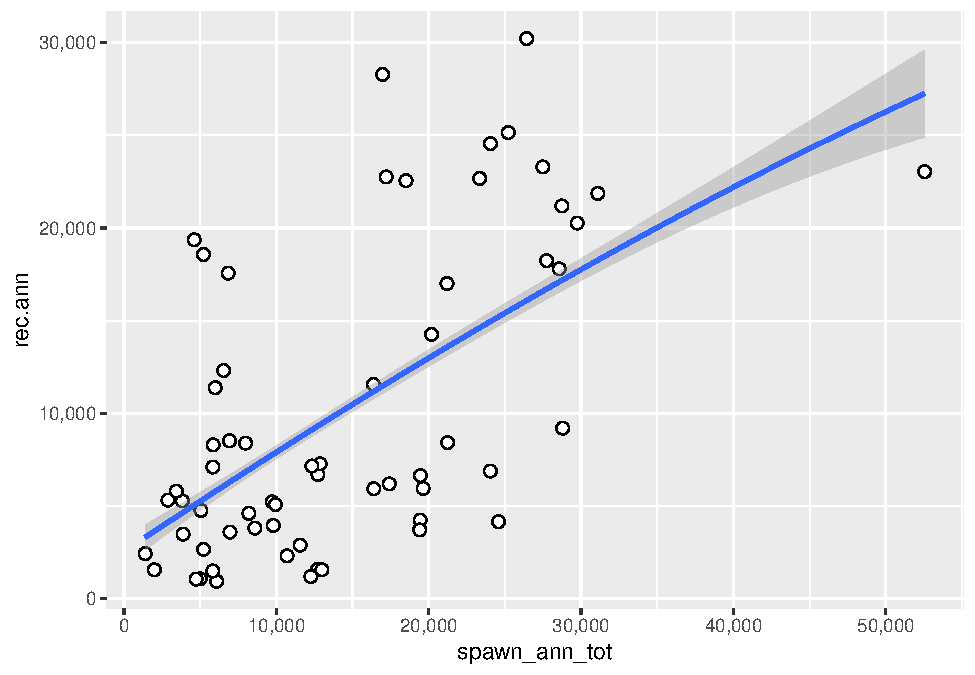
\includegraphics{3_Vis_CCM_Causal_Vars_files/figure-latex/unnamed-chunk-4-1.pdf}

\begin{Shaded}
\begin{Highlighting}[]
\FunctionTok{ggplot}\NormalTok{(df, }\FunctionTok{aes}\NormalTok{(}\AttributeTok{x =}\NormalTok{ ESU\_rec4n, }\AttributeTok{color =}\NormalTok{ domain, }\AttributeTok{fill =}\NormalTok{ domain )) }\SpecialCharTok{+}
  \FunctionTok{geom\_histogram}\NormalTok{(}\AttributeTok{position =} \StringTok{"identity"}\NormalTok{, }\AttributeTok{binwidth =} \FloatTok{0.02}\NormalTok{, }\AttributeTok{alpha =} \FloatTok{0.4}\NormalTok{) }\SpecialCharTok{+}
  \FunctionTok{geom\_density}\NormalTok{(}\AttributeTok{alpha =} \FloatTok{0.4}\NormalTok{) }\SpecialCharTok{+}
  \FunctionTok{geom\_vline}\NormalTok{(}\FunctionTok{aes}\NormalTok{(}\AttributeTok{xintercept =}\NormalTok{ mu\_ESU, }\AttributeTok{color =}\NormalTok{ domain),}
             \AttributeTok{linetype =} \StringTok{"dashed"}\NormalTok{) }\SpecialCharTok{+}
  \FunctionTok{theme}\NormalTok{(}\AttributeTok{legend.position =} \StringTok{"top"}\NormalTok{) }\SpecialCharTok{+}
  \FunctionTok{scale\_color\_manual}\NormalTok{(}\AttributeTok{values=}\FunctionTok{c}\NormalTok{(}\StringTok{"\#FFC300"}\NormalTok{, }\StringTok{"\#2E86C1"}\NormalTok{, }\StringTok{"\#CB4335"}\NormalTok{)) }\SpecialCharTok{+}
  \FunctionTok{scale\_fill\_manual}\NormalTok{(}\AttributeTok{values=}\FunctionTok{c}\NormalTok{(}\StringTok{"\#FFC300"}\NormalTok{, }\StringTok{"\#2E86C1"}\NormalTok{, }\StringTok{"\#CB4335"}\NormalTok{))}
\end{Highlighting}
\end{Shaded}

\begin{verbatim}
## Warning: Removed 22 rows containing non-finite values (stat_bin).
\end{verbatim}

\begin{verbatim}
## Warning: Removed 22 rows containing non-finite values (stat_density).
\end{verbatim}

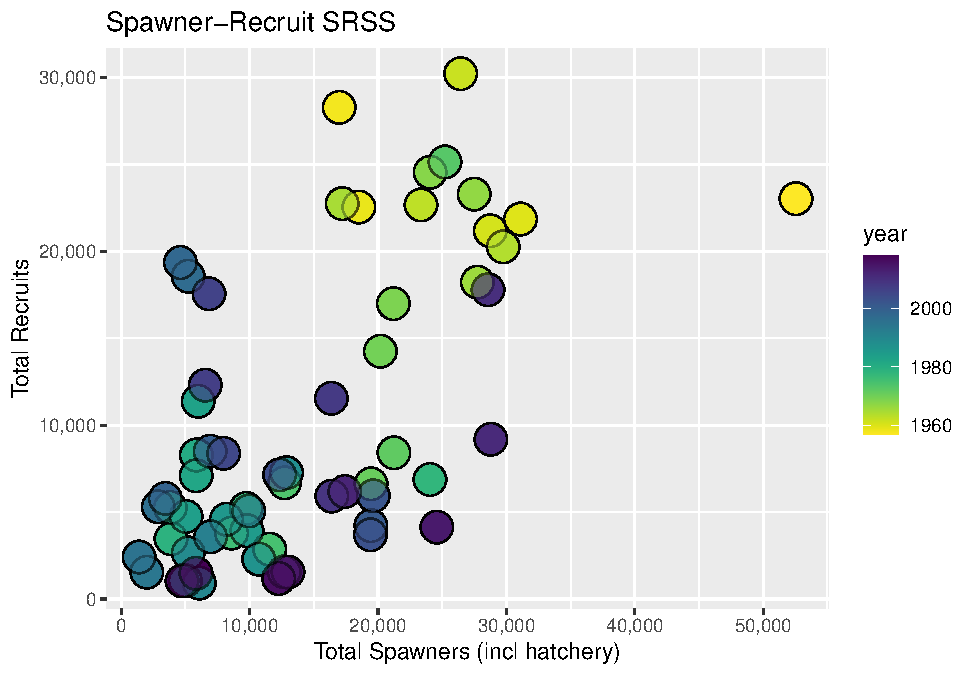
\includegraphics{3_Vis_CCM_Causal_Vars_files/figure-latex/unnamed-chunk-4-2.pdf}

\begin{Shaded}
\begin{Highlighting}[]
\FunctionTok{ggplot}\NormalTok{(df, }\FunctionTok{aes}\NormalTok{(}\AttributeTok{x =}\NormalTok{ ESU\_rec4n, }\AttributeTok{color =}\NormalTok{ domain, }\AttributeTok{fill =}\NormalTok{ domain )) }\SpecialCharTok{+} 
  \FunctionTok{geom\_histogram}\NormalTok{(}\AttributeTok{position =} \StringTok{"identity"}\NormalTok{, }\AttributeTok{binwidth =} \FloatTok{0.02}\NormalTok{, }\AttributeTok{alpha =} \FloatTok{0.4}\NormalTok{) }\SpecialCharTok{+}
  \FunctionTok{geom\_density}\NormalTok{(}\AttributeTok{alpha =} \FloatTok{0.4}\NormalTok{) }\SpecialCharTok{+}
  \FunctionTok{scale\_color\_manual}\NormalTok{(}\AttributeTok{values=}\FunctionTok{c}\NormalTok{(}\StringTok{"\#FFC300"}\NormalTok{, }\StringTok{"\#2E86C1"}\NormalTok{, }\StringTok{"\#CB4335"}\NormalTok{)) }\SpecialCharTok{+}
  \FunctionTok{scale\_fill\_manual}\NormalTok{(}\AttributeTok{values=}\FunctionTok{c}\NormalTok{(}\StringTok{"\#FFC300"}\NormalTok{, }\StringTok{"\#2E86C1"}\NormalTok{, }\StringTok{"\#CB4335"}\NormalTok{)) }\SpecialCharTok{+}
  \FunctionTok{facet\_grid}\NormalTok{(domain }\SpecialCharTok{\textasciitilde{}}\NormalTok{ .) }\SpecialCharTok{+}
  \FunctionTok{geom\_vline}\NormalTok{(}\FunctionTok{aes}\NormalTok{(}\AttributeTok{xintercept =}\NormalTok{ mu\_ESU, }\AttributeTok{color =}\NormalTok{ domain),}
            \AttributeTok{lty =} \StringTok{"11"}\NormalTok{, }\AttributeTok{lwd =} \FloatTok{1.5}\NormalTok{) }\SpecialCharTok{+}
  \FunctionTok{theme\_bw}\NormalTok{() }\SpecialCharTok{+}
  \FunctionTok{theme}\NormalTok{(}\AttributeTok{axis.ticks.y =} \FunctionTok{element\_blank}\NormalTok{(),}
        \AttributeTok{axis.text.y =} \FunctionTok{element\_blank}\NormalTok{()) }\SpecialCharTok{+}
  \FunctionTok{ylab}\NormalTok{(}\StringTok{"Frequency"}\NormalTok{) }\SpecialCharTok{+} \FunctionTok{xlab}\NormalTok{(}\StringTok{"Rho (correlation coefficient, obs vs pred)"}\NormalTok{) }\SpecialCharTok{+}
  \FunctionTok{xlim}\NormalTok{(}\FunctionTok{c}\NormalTok{(}\DecValTok{0}\NormalTok{, }\DecValTok{1}\NormalTok{))}
\end{Highlighting}
\end{Shaded}

\begin{verbatim}
## Warning: Removed 22 rows containing non-finite values (stat_bin).

## Warning: Removed 22 rows containing non-finite values (stat_density).
\end{verbatim}

\begin{verbatim}
## Warning: Removed 6 rows containing missing values (geom_bar).
\end{verbatim}

\includegraphics{3_Vis_CCM_Causal_Vars_files/figure-latex/unnamed-chunk-4-3.pdf}

\hypertarget{are-predators-important-drivers-of-salmon-recruitment-yes-numerous-predator-time-series-exceed-ccm-thresholds-of-rho-0-and-increasing-with-library-size.-magnitude-of-correlation-coeffient-between-predator-putative-causal-variables-those-predicted-by-salmon-recuitment-levels-is-on-average-higher-than-humn-or-ocean-variables.-indicating-that-several-predator-pcv-left-a-strong-imprint-on-salmon-dynamics}{%
\subsubsection{Are predators important drivers of salmon recruitment?
Yes, numerous predator time series exceed CCM thresholds of rho
\textgreater{} 0 and increasing with library size. Magnitude of
correlation coeffient between predator putative causal variables those
predicted by salmon recuitment levels is, on average higher than humn or
ocean variables. indicating that several predator pcv left a strong
imprint on salmon
dynamics}\label{are-predators-important-drivers-of-salmon-recruitment-yes-numerous-predator-time-series-exceed-ccm-thresholds-of-rho-0-and-increasing-with-library-size.-magnitude-of-correlation-coeffient-between-predator-putative-causal-variables-those-predicted-by-salmon-recuitment-levels-is-on-average-higher-than-humn-or-ocean-variables.-indicating-that-several-predator-pcv-left-a-strong-imprint-on-salmon-dynamics}}

\hypertarget{within-each-domain-how-do-the-various-categories-stack-up}{%
\subsubsection{Within each domain, how do the various categories stack
up}\label{within-each-domain-how-do-the-various-categories-stack-up}}

\begin{Shaded}
\begin{Highlighting}[]
\CommentTok{\# roughly simlar mean rho: ssl slightly higher}

\NormalTok{ocean }\OtherTok{\textless{}{-}}\NormalTok{ df }\SpecialCharTok{\%\textgreater{}\%} 
  \FunctionTok{filter}\NormalTok{(domain }\SpecialCharTok{==} \StringTok{"ocean"}\NormalTok{) }\SpecialCharTok{\%\textgreater{}\%} 
  \FunctionTok{group\_by}\NormalTok{(cat) }\SpecialCharTok{\%\textgreater{}\%} 
  \FunctionTok{mutate}\NormalTok{(}\AttributeTok{mu =} \FunctionTok{mean}\NormalTok{(ESU\_rec4n, }\AttributeTok{na.rm=}\ConstantTok{TRUE}\NormalTok{)) }\SpecialCharTok{\%\textgreater{}\%}
  \FunctionTok{ungroup}\NormalTok{()}

\NormalTok{ocean}\SpecialCharTok{$}\NormalTok{cat }\OtherTok{=} \FunctionTok{factor}\NormalTok{(ocean}\SpecialCharTok{$}\NormalTok{cat, }\AttributeTok{levels=}\FunctionTok{c}\NormalTok{(}\StringTok{\textquotesingle{}pdo\textquotesingle{}}\NormalTok{,}\StringTok{\textquotesingle{}arc\textquotesingle{}}\NormalTok{,}\StringTok{\textquotesingle{}upw\textquotesingle{}}\NormalTok{,}\StringTok{\textquotesingle{}npgo\textquotesingle{}}\NormalTok{))}

\FunctionTok{ggplot}\NormalTok{(ocean, }\FunctionTok{aes}\NormalTok{(}\AttributeTok{x =}\NormalTok{ ESU\_rec4n, }\AttributeTok{color =}\NormalTok{ cat, }\AttributeTok{fill =}\NormalTok{ cat)) }\SpecialCharTok{+} 
  \FunctionTok{geom\_histogram}\NormalTok{(}\AttributeTok{position =} \StringTok{"identity"}\NormalTok{, }\AttributeTok{binwidth =} \FloatTok{0.02}\NormalTok{, }\AttributeTok{alpha =} \FloatTok{0.7}\NormalTok{) }\SpecialCharTok{+}
  \FunctionTok{scale\_color\_manual}\NormalTok{(}\AttributeTok{values =} \FunctionTok{colorRampPalette}\NormalTok{(}\FunctionTok{brewer.pal}\NormalTok{(}\DecValTok{9}\NormalTok{, }\StringTok{"Blues"}\NormalTok{))(}\DecValTok{8}\NormalTok{)[}\DecValTok{4}\SpecialCharTok{:}\DecValTok{7}\NormalTok{]) }\SpecialCharTok{+}
  \FunctionTok{scale\_fill\_manual}\NormalTok{(}\AttributeTok{values =} \FunctionTok{colorRampPalette}\NormalTok{(}\FunctionTok{brewer.pal}\NormalTok{(}\DecValTok{9}\NormalTok{, }\StringTok{"Blues"}\NormalTok{))(}\DecValTok{8}\NormalTok{)[}\DecValTok{4}\SpecialCharTok{:}\DecValTok{7}\NormalTok{]) }\SpecialCharTok{+}
  \FunctionTok{geom\_vline}\NormalTok{(}\FunctionTok{aes}\NormalTok{(}\AttributeTok{xintercept =}\NormalTok{ mu, }\AttributeTok{color =}\NormalTok{ cat),}
             \AttributeTok{linetype =} \StringTok{"dashed"}\NormalTok{) }\SpecialCharTok{+}
  \FunctionTok{geom\_density}\NormalTok{(}\AttributeTok{alpha =} \FloatTok{0.4}\NormalTok{) }\SpecialCharTok{+} \FunctionTok{facet\_grid}\NormalTok{(cat }\SpecialCharTok{\textasciitilde{}}\NormalTok{ .) }\SpecialCharTok{+}
  \FunctionTok{theme\_bw}\NormalTok{() }\SpecialCharTok{+}
  \FunctionTok{theme}\NormalTok{(}\AttributeTok{axis.ticks.y =} \FunctionTok{element\_blank}\NormalTok{(),}
        \AttributeTok{axis.text.y =} \FunctionTok{element\_blank}\NormalTok{()) }\SpecialCharTok{+}
  \FunctionTok{ylab}\NormalTok{(}\StringTok{"Frequency"}\NormalTok{) }\SpecialCharTok{+} \FunctionTok{xlab}\NormalTok{(}\StringTok{"Rho (correlation coefficient, obs vs pred)"}\NormalTok{) }\SpecialCharTok{+}
  \FunctionTok{xlim}\NormalTok{(}\FunctionTok{c}\NormalTok{(}\DecValTok{0}\NormalTok{, }\DecValTok{1}\NormalTok{))}
\end{Highlighting}
\end{Shaded}

\begin{verbatim}
## Warning: Removed 8 rows containing missing values (geom_bar).
\end{verbatim}

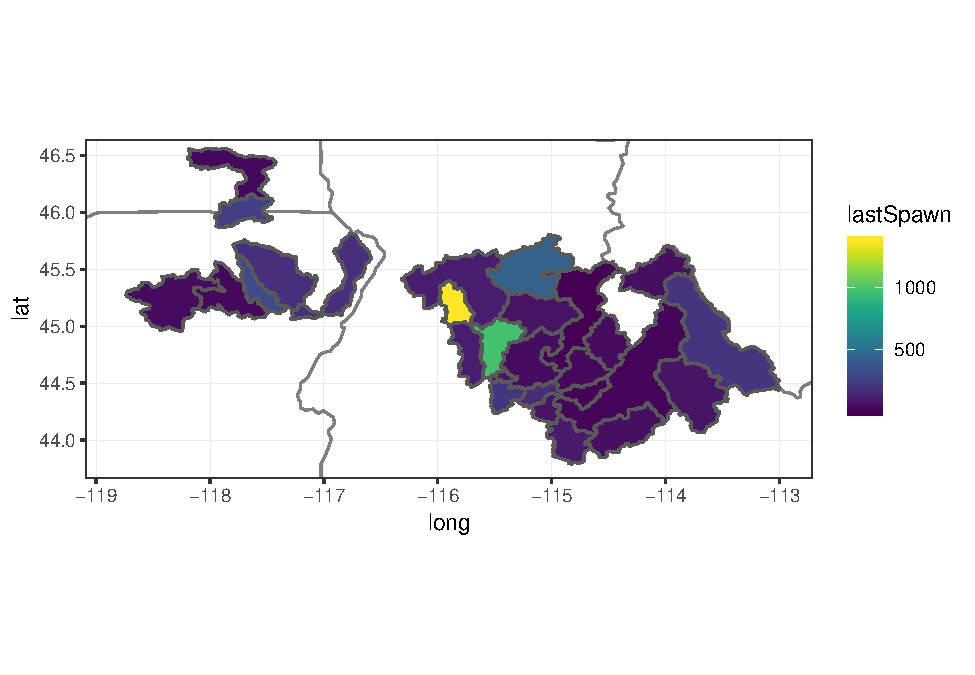
\includegraphics{3_Vis_CCM_Causal_Vars_files/figure-latex/unnamed-chunk-5-1.pdf}
\#\#\#\# For rec4, NPGO higher than other ocean vars

\begin{Shaded}
\begin{Highlighting}[]
\NormalTok{predator }\OtherTok{\textless{}{-}}\NormalTok{ df }\SpecialCharTok{\%\textgreater{}\%} 
  \FunctionTok{filter}\NormalTok{(domain }\SpecialCharTok{==} \StringTok{"predator"}\NormalTok{) }\SpecialCharTok{\%\textgreater{}\%} 
  \FunctionTok{group\_by}\NormalTok{(cat) }\SpecialCharTok{\%\textgreater{}\%} 
  \FunctionTok{mutate}\NormalTok{(}\AttributeTok{mu =} \FunctionTok{mean}\NormalTok{(ESU\_rec4n, }\AttributeTok{na.rm=}\ConstantTok{TRUE}\NormalTok{)) }\SpecialCharTok{\%\textgreater{}\%}
  \FunctionTok{ungroup}\NormalTok{()}

\NormalTok{predator}\SpecialCharTok{$}\NormalTok{cat }\OtherTok{=} \FunctionTok{factor}\NormalTok{(predator}\SpecialCharTok{$}\NormalTok{cat, }\AttributeTok{levels=}\FunctionTok{c}\NormalTok{(}\StringTok{\textquotesingle{}orca\textquotesingle{}}\NormalTok{,}\StringTok{\textquotesingle{}csl\textquotesingle{}}\NormalTok{,}\StringTok{\textquotesingle{}ssl\textquotesingle{}}\NormalTok{))}

\FunctionTok{ggplot}\NormalTok{(predator, }\FunctionTok{aes}\NormalTok{(}\AttributeTok{x =}\NormalTok{ ESU\_rec4n, }\AttributeTok{color =}\NormalTok{ cat, }\AttributeTok{fill =}\NormalTok{ cat)) }\SpecialCharTok{+} 
  \FunctionTok{geom\_histogram}\NormalTok{(}\AttributeTok{position =} \StringTok{"identity"}\NormalTok{, }\AttributeTok{binwidth =} \FloatTok{0.02}\NormalTok{, }\AttributeTok{alpha =} \FloatTok{0.7}\NormalTok{) }\SpecialCharTok{+}
  \FunctionTok{scale\_color\_manual}\NormalTok{(}\AttributeTok{values =} \FunctionTok{colorRampPalette}\NormalTok{(}\FunctionTok{brewer.pal}\NormalTok{(}\DecValTok{9}\NormalTok{, }\StringTok{"Reds"}\NormalTok{))(}\DecValTok{6}\NormalTok{)[}\DecValTok{2}\SpecialCharTok{:}\DecValTok{4}\NormalTok{]) }\SpecialCharTok{+}
  \FunctionTok{scale\_fill\_manual}\NormalTok{(}\AttributeTok{values =} \FunctionTok{colorRampPalette}\NormalTok{(}\FunctionTok{brewer.pal}\NormalTok{(}\DecValTok{9}\NormalTok{, }\StringTok{"Reds"}\NormalTok{))(}\DecValTok{6}\NormalTok{)[}\DecValTok{2}\SpecialCharTok{:}\DecValTok{4}\NormalTok{]) }\SpecialCharTok{+}
  \FunctionTok{geom\_vline}\NormalTok{(}\FunctionTok{aes}\NormalTok{(}\AttributeTok{xintercept =}\NormalTok{ mu, }\AttributeTok{color =}\NormalTok{ cat),}
             \AttributeTok{linetype =} \StringTok{"dashed"}\NormalTok{) }\SpecialCharTok{+}
  \FunctionTok{geom\_density}\NormalTok{(}\AttributeTok{alpha =} \FloatTok{0.4}\NormalTok{) }\SpecialCharTok{+} \FunctionTok{facet\_grid}\NormalTok{(cat }\SpecialCharTok{\textasciitilde{}}\NormalTok{ .) }\SpecialCharTok{+}
  \FunctionTok{theme\_bw}\NormalTok{() }\SpecialCharTok{+}
  \FunctionTok{theme}\NormalTok{(}\AttributeTok{axis.ticks.y =} \FunctionTok{element\_blank}\NormalTok{(),}
        \AttributeTok{axis.text.y =} \FunctionTok{element\_blank}\NormalTok{()) }\SpecialCharTok{+}
  \FunctionTok{ylab}\NormalTok{(}\StringTok{"Frequency"}\NormalTok{) }\SpecialCharTok{+} \FunctionTok{xlab}\NormalTok{(}\StringTok{"Rho (correlation coefficient, obs vs pred)"}\NormalTok{) }\SpecialCharTok{+}
  \FunctionTok{xlim}\NormalTok{(}\FunctionTok{c}\NormalTok{(}\DecValTok{0}\NormalTok{, }\DecValTok{1}\NormalTok{))}
\end{Highlighting}
\end{Shaded}

\begin{verbatim}
## Warning: Removed 8 rows containing non-finite values (stat_bin).
\end{verbatim}

\begin{verbatim}
## Warning: Removed 8 rows containing non-finite values (stat_density).
\end{verbatim}

\begin{verbatim}
## Warning: Removed 6 rows containing missing values (geom_bar).
\end{verbatim}

\includegraphics{3_Vis_CCM_Causal_Vars_files/figure-latex/unnamed-chunk-6-1.pdf}
\#\#\#\# For rec4, SSL higher than other pred vars

\begin{Shaded}
\begin{Highlighting}[]
\NormalTok{human }\OtherTok{\textless{}{-}}\NormalTok{ df }\SpecialCharTok{\%\textgreater{}\%} 
  \FunctionTok{filter}\NormalTok{(domain }\SpecialCharTok{==} \StringTok{"human"}\NormalTok{) }\SpecialCharTok{\%\textgreater{}\%} 
  \FunctionTok{group\_by}\NormalTok{(cat) }\SpecialCharTok{\%\textgreater{}\%} 
  \FunctionTok{mutate}\NormalTok{(}\AttributeTok{mu =} \FunctionTok{mean}\NormalTok{(ESU\_rec4n, }\AttributeTok{na.rm=}\ConstantTok{TRUE}\NormalTok{)) }\SpecialCharTok{\%\textgreater{}\%}
  \FunctionTok{ungroup}\NormalTok{()}

\NormalTok{human}\SpecialCharTok{$}\NormalTok{cat }\OtherTok{=} \FunctionTok{factor}\NormalTok{(human}\SpecialCharTok{$}\NormalTok{cat, }\AttributeTok{levels=}\FunctionTok{c}\NormalTok{(}\StringTok{\textquotesingle{}hatch\textquotesingle{}}\NormalTok{,}\StringTok{\textquotesingle{}harv\textquotesingle{}}\NormalTok{))}

\FunctionTok{ggplot}\NormalTok{(human, }\FunctionTok{aes}\NormalTok{(}\AttributeTok{x =}\NormalTok{ ESU\_rec4n, }\AttributeTok{color =}\NormalTok{ cat, }\AttributeTok{fill =}\NormalTok{ cat)) }\SpecialCharTok{+} 
  \FunctionTok{geom\_histogram}\NormalTok{(}\AttributeTok{position =} \StringTok{"identity"}\NormalTok{, }\AttributeTok{binwidth =} \FloatTok{0.02}\NormalTok{, }\AttributeTok{alpha =} \FloatTok{0.7}\NormalTok{) }\SpecialCharTok{+}
  \FunctionTok{scale\_color\_manual}\NormalTok{(}\AttributeTok{values =} \FunctionTok{c}\NormalTok{(}\StringTok{"\#FFC300"}\NormalTok{ , }\StringTok{"\#FFDA60"}\NormalTok{)) }\SpecialCharTok{+}
  \FunctionTok{scale\_fill\_manual}\NormalTok{(}\AttributeTok{values =} \FunctionTok{c}\NormalTok{(}\StringTok{"\#FFC300"}\NormalTok{ , }\StringTok{"\#FFDA60"}\NormalTok{)) }\SpecialCharTok{+}
  \FunctionTok{geom\_vline}\NormalTok{(}\FunctionTok{aes}\NormalTok{(}\AttributeTok{xintercept =}\NormalTok{ mu, }\AttributeTok{color =}\NormalTok{ cat),}
             \AttributeTok{linetype =} \StringTok{"dashed"}\NormalTok{) }\SpecialCharTok{+}
  \FunctionTok{geom\_density}\NormalTok{(}\AttributeTok{alpha =} \FloatTok{0.4}\NormalTok{) }\SpecialCharTok{+} \FunctionTok{facet\_grid}\NormalTok{(cat }\SpecialCharTok{\textasciitilde{}}\NormalTok{ .) }\SpecialCharTok{+}
  \FunctionTok{theme\_bw}\NormalTok{() }\SpecialCharTok{+}
  \FunctionTok{theme}\NormalTok{(}\AttributeTok{axis.ticks.y =} \FunctionTok{element\_blank}\NormalTok{(),}
        \AttributeTok{axis.text.y =} \FunctionTok{element\_blank}\NormalTok{()) }\SpecialCharTok{+}
  \FunctionTok{ylab}\NormalTok{(}\StringTok{"Frequency"}\NormalTok{) }\SpecialCharTok{+} \FunctionTok{xlab}\NormalTok{(}\StringTok{"Rho (correlation coefficient, obs vs pred)"}\NormalTok{) }\SpecialCharTok{+}
  \FunctionTok{xlim}\NormalTok{(}\FunctionTok{c}\NormalTok{(}\DecValTok{0}\NormalTok{, }\DecValTok{1}\NormalTok{))}
\end{Highlighting}
\end{Shaded}

\begin{verbatim}
## Warning: Removed 14 rows containing non-finite values (stat_bin).
\end{verbatim}

\begin{verbatim}
## Warning: Removed 14 rows containing non-finite values (stat_density).
\end{verbatim}

\begin{verbatim}
## Warning: Removed 4 rows containing missing values (geom_bar).
\end{verbatim}

\includegraphics{3_Vis_CCM_Causal_Vars_files/figure-latex/unnamed-chunk-7-1.pdf}
\#\#\#\# For rec4, harvest higher than hatchery

Rec 5

\begin{Shaded}
\begin{Highlighting}[]
\FunctionTok{ggplot}\NormalTok{(df, }\FunctionTok{aes}\NormalTok{(}\AttributeTok{x =}\NormalTok{ ESU\_rec5n, }\AttributeTok{color =}\NormalTok{ domain, }\AttributeTok{fill =}\NormalTok{ domain )) }\SpecialCharTok{+}
  \FunctionTok{geom\_histogram}\NormalTok{(}\AttributeTok{position =} \StringTok{"identity"}\NormalTok{, }\AttributeTok{binwidth =} \FloatTok{0.02}\NormalTok{, }\AttributeTok{alpha =} \FloatTok{0.4}\NormalTok{) }\SpecialCharTok{+}
  \FunctionTok{geom\_density}\NormalTok{(}\AttributeTok{alpha =} \FloatTok{0.4}\NormalTok{) }\SpecialCharTok{+}
  \FunctionTok{geom\_vline}\NormalTok{(}\FunctionTok{aes}\NormalTok{(}\AttributeTok{xintercept =}\NormalTok{ mu\_ESU, }\AttributeTok{color =}\NormalTok{ domain),}
             \AttributeTok{linetype =} \StringTok{"dashed"}\NormalTok{) }\SpecialCharTok{+}
  \FunctionTok{theme}\NormalTok{(}\AttributeTok{legend.position =} \StringTok{"top"}\NormalTok{) }\SpecialCharTok{+}
  \FunctionTok{scale\_color\_manual}\NormalTok{(}\AttributeTok{values=}\FunctionTok{c}\NormalTok{(}\StringTok{"\#FFC300"}\NormalTok{, }\StringTok{"\#2E86C1"}\NormalTok{, }\StringTok{"\#CB4335"}\NormalTok{)) }\SpecialCharTok{+}
  \FunctionTok{scale\_fill\_manual}\NormalTok{(}\AttributeTok{values=}\FunctionTok{c}\NormalTok{(}\StringTok{"\#FFC300"}\NormalTok{, }\StringTok{"\#2E86C1"}\NormalTok{, }\StringTok{"\#CB4335"}\NormalTok{))}
\end{Highlighting}
\end{Shaded}

\includegraphics{3_Vis_CCM_Causal_Vars_files/figure-latex/unnamed-chunk-8-1.pdf}

\begin{Shaded}
\begin{Highlighting}[]
\FunctionTok{ggplot}\NormalTok{(df, }\FunctionTok{aes}\NormalTok{(}\AttributeTok{x =}\NormalTok{ ESU\_rec5n, }\AttributeTok{color =}\NormalTok{ domain, }\AttributeTok{fill =}\NormalTok{ domain )) }\SpecialCharTok{+} 
  \FunctionTok{geom\_histogram}\NormalTok{(}\AttributeTok{position =} \StringTok{"identity"}\NormalTok{, }\AttributeTok{binwidth =} \FloatTok{0.02}\NormalTok{, }\AttributeTok{alpha =} \FloatTok{0.4}\NormalTok{) }\SpecialCharTok{+}
  \FunctionTok{geom\_density}\NormalTok{(}\AttributeTok{alpha =} \FloatTok{0.4}\NormalTok{) }\SpecialCharTok{+}
  \FunctionTok{scale\_color\_manual}\NormalTok{(}\AttributeTok{values=}\FunctionTok{c}\NormalTok{(}\StringTok{"\#FFC300"}\NormalTok{, }\StringTok{"\#2E86C1"}\NormalTok{, }\StringTok{"\#CB4335"}\NormalTok{)) }\SpecialCharTok{+}
  \FunctionTok{scale\_fill\_manual}\NormalTok{(}\AttributeTok{values=}\FunctionTok{c}\NormalTok{(}\StringTok{"\#FFC300"}\NormalTok{, }\StringTok{"\#2E86C1"}\NormalTok{, }\StringTok{"\#CB4335"}\NormalTok{)) }\SpecialCharTok{+}
  \FunctionTok{facet\_grid}\NormalTok{(domain }\SpecialCharTok{\textasciitilde{}}\NormalTok{ .) }\SpecialCharTok{+}
  \FunctionTok{geom\_vline}\NormalTok{(}\FunctionTok{aes}\NormalTok{(}\AttributeTok{xintercept =}\NormalTok{ mu\_ESU, }\AttributeTok{color =}\NormalTok{ domain),}
            \AttributeTok{lty =} \StringTok{"11"}\NormalTok{, }\AttributeTok{lwd =} \FloatTok{1.5}\NormalTok{) }\SpecialCharTok{+}
  \FunctionTok{theme\_bw}\NormalTok{() }\SpecialCharTok{+}
  \FunctionTok{theme}\NormalTok{(}\AttributeTok{axis.ticks.y =} \FunctionTok{element\_blank}\NormalTok{(),}
        \AttributeTok{axis.text.y =} \FunctionTok{element\_blank}\NormalTok{()) }\SpecialCharTok{+}
  \FunctionTok{ylab}\NormalTok{(}\StringTok{"Frequency"}\NormalTok{) }\SpecialCharTok{+} \FunctionTok{xlab}\NormalTok{(}\StringTok{"Rho (correlation coefficient, obs vs pred)"}\NormalTok{) }\SpecialCharTok{+}
  \FunctionTok{xlim}\NormalTok{(}\FunctionTok{c}\NormalTok{(}\DecValTok{0}\NormalTok{, }\DecValTok{1}\NormalTok{))}
\end{Highlighting}
\end{Shaded}

\begin{verbatim}
## Warning: Removed 6 rows containing missing values (geom_bar).
\end{verbatim}

\includegraphics{3_Vis_CCM_Causal_Vars_files/figure-latex/unnamed-chunk-8-2.pdf}

\hypertarget{compared-to-rec4-the-rec5-mean-rho-for-predators-is-similar-but-there-is-far-more-right-skew-or-a-small-number-of-predator-vars-with-very-high-rh0}{%
\subsubsection{Compared to rec4, the rec5 mean rho for predators is
similar but there is far more right-skew, or a small number of predator
vars with very high
rh0}\label{compared-to-rec4-the-rec5-mean-rho-for-predators-is-similar-but-there-is-far-more-right-skew-or-a-small-number-of-predator-vars-with-very-high-rh0}}

\hypertarget{within-each-domain-how-do-the-various-categories-stack-up-1}{%
\subsubsection{Within each domain, how do the various categories stack
up}\label{within-each-domain-how-do-the-various-categories-stack-up-1}}

\begin{Shaded}
\begin{Highlighting}[]
\NormalTok{ocean }\OtherTok{\textless{}{-}}\NormalTok{ df }\SpecialCharTok{\%\textgreater{}\%} 
  \FunctionTok{filter}\NormalTok{(domain }\SpecialCharTok{==} \StringTok{"ocean"}\NormalTok{) }\SpecialCharTok{\%\textgreater{}\%} 
  \FunctionTok{group\_by}\NormalTok{(cat) }\SpecialCharTok{\%\textgreater{}\%} 
  \FunctionTok{mutate}\NormalTok{(}\AttributeTok{mu =} \FunctionTok{mean}\NormalTok{(ESU\_rec5n, }\AttributeTok{na.rm=}\ConstantTok{TRUE}\NormalTok{)) }\SpecialCharTok{\%\textgreater{}\%}
  \FunctionTok{ungroup}\NormalTok{()}

\NormalTok{ocean}\SpecialCharTok{$}\NormalTok{cat }\OtherTok{=} \FunctionTok{factor}\NormalTok{(ocean}\SpecialCharTok{$}\NormalTok{cat, }\AttributeTok{levels=}\FunctionTok{c}\NormalTok{(}\StringTok{\textquotesingle{}pdo\textquotesingle{}}\NormalTok{,}\StringTok{\textquotesingle{}upw\textquotesingle{}}\NormalTok{,}\StringTok{\textquotesingle{}arc\textquotesingle{}}\NormalTok{,}\StringTok{\textquotesingle{}npgo\textquotesingle{}}\NormalTok{))}

\FunctionTok{ggplot}\NormalTok{(ocean, }\FunctionTok{aes}\NormalTok{(}\AttributeTok{x =}\NormalTok{ ESU\_rec5n, }\AttributeTok{color =}\NormalTok{ cat, }\AttributeTok{fill =}\NormalTok{ cat)) }\SpecialCharTok{+} 
  \FunctionTok{geom\_histogram}\NormalTok{(}\AttributeTok{position =} \StringTok{"identity"}\NormalTok{, }\AttributeTok{binwidth =} \FloatTok{0.02}\NormalTok{, }\AttributeTok{alpha =} \FloatTok{0.7}\NormalTok{) }\SpecialCharTok{+}
  \FunctionTok{scale\_color\_manual}\NormalTok{(}\AttributeTok{values =} \FunctionTok{colorRampPalette}\NormalTok{(}\FunctionTok{brewer.pal}\NormalTok{(}\DecValTok{9}\NormalTok{, }\StringTok{"Blues"}\NormalTok{))(}\DecValTok{8}\NormalTok{)[}\DecValTok{4}\SpecialCharTok{:}\DecValTok{7}\NormalTok{]) }\SpecialCharTok{+}
  \FunctionTok{scale\_fill\_manual}\NormalTok{(}\AttributeTok{values =} \FunctionTok{colorRampPalette}\NormalTok{(}\FunctionTok{brewer.pal}\NormalTok{(}\DecValTok{9}\NormalTok{, }\StringTok{"Blues"}\NormalTok{))(}\DecValTok{8}\NormalTok{)[}\DecValTok{4}\SpecialCharTok{:}\DecValTok{7}\NormalTok{]) }\SpecialCharTok{+}
  \FunctionTok{geom\_vline}\NormalTok{(}\FunctionTok{aes}\NormalTok{(}\AttributeTok{xintercept =}\NormalTok{ mu, }\AttributeTok{color =}\NormalTok{ cat),}
             \AttributeTok{linetype =} \StringTok{"dashed"}\NormalTok{) }\SpecialCharTok{+}
  \FunctionTok{geom\_density}\NormalTok{(}\AttributeTok{alpha =} \FloatTok{0.4}\NormalTok{) }\SpecialCharTok{+} \FunctionTok{facet\_grid}\NormalTok{(cat }\SpecialCharTok{\textasciitilde{}}\NormalTok{ .) }\SpecialCharTok{+}
  \FunctionTok{theme\_bw}\NormalTok{() }\SpecialCharTok{+}
  \FunctionTok{theme}\NormalTok{(}\AttributeTok{axis.ticks.y =} \FunctionTok{element\_blank}\NormalTok{(),}
        \AttributeTok{axis.text.y =} \FunctionTok{element\_blank}\NormalTok{()) }\SpecialCharTok{+}
  \FunctionTok{ylab}\NormalTok{(}\StringTok{"Frequency"}\NormalTok{) }\SpecialCharTok{+} \FunctionTok{xlab}\NormalTok{(}\StringTok{"Rho (correlation coefficient, obs vs pred)"}\NormalTok{) }\SpecialCharTok{+}
  \FunctionTok{xlim}\NormalTok{(}\FunctionTok{c}\NormalTok{(}\DecValTok{0}\NormalTok{, }\DecValTok{1}\NormalTok{))}
\end{Highlighting}
\end{Shaded}

\begin{verbatim}
## Warning: Removed 8 rows containing missing values (geom_bar).
\end{verbatim}

\includegraphics{3_Vis_CCM_Causal_Vars_files/figure-latex/unnamed-chunk-9-1.pdf}
\#\#\#\# For rec5, NPGO remains higher than other ocean vars

\begin{Shaded}
\begin{Highlighting}[]
\NormalTok{predator }\OtherTok{\textless{}{-}}\NormalTok{ df }\SpecialCharTok{\%\textgreater{}\%} 
  \FunctionTok{filter}\NormalTok{(domain }\SpecialCharTok{==} \StringTok{"predator"}\NormalTok{) }\SpecialCharTok{\%\textgreater{}\%} 
  \FunctionTok{group\_by}\NormalTok{(cat) }\SpecialCharTok{\%\textgreater{}\%} 
  \FunctionTok{mutate}\NormalTok{(}\AttributeTok{mu =} \FunctionTok{mean}\NormalTok{(ESU\_rec5n, }\AttributeTok{na.rm=}\ConstantTok{TRUE}\NormalTok{)) }\SpecialCharTok{\%\textgreater{}\%}
  \FunctionTok{ungroup}\NormalTok{()}

\NormalTok{predator}\SpecialCharTok{$}\NormalTok{cat }\OtherTok{=} \FunctionTok{factor}\NormalTok{(predator}\SpecialCharTok{$}\NormalTok{cat, }\AttributeTok{levels=}\FunctionTok{c}\NormalTok{(}\StringTok{\textquotesingle{}orca\textquotesingle{}}\NormalTok{,}\StringTok{\textquotesingle{}csl\textquotesingle{}}\NormalTok{,}\StringTok{\textquotesingle{}ssl\textquotesingle{}}\NormalTok{))}

\FunctionTok{ggplot}\NormalTok{(predator, }\FunctionTok{aes}\NormalTok{(}\AttributeTok{x =}\NormalTok{ ESU\_rec5n, }\AttributeTok{color =}\NormalTok{ cat, }\AttributeTok{fill =}\NormalTok{ cat)) }\SpecialCharTok{+} 
  \FunctionTok{geom\_histogram}\NormalTok{(}\AttributeTok{position =} \StringTok{"identity"}\NormalTok{, }\AttributeTok{binwidth =} \FloatTok{0.02}\NormalTok{, }\AttributeTok{alpha =} \FloatTok{0.7}\NormalTok{) }\SpecialCharTok{+}
  \FunctionTok{scale\_color\_manual}\NormalTok{(}\AttributeTok{values =} \FunctionTok{colorRampPalette}\NormalTok{(}\FunctionTok{brewer.pal}\NormalTok{(}\DecValTok{9}\NormalTok{, }\StringTok{"Reds"}\NormalTok{))(}\DecValTok{6}\NormalTok{)[}\DecValTok{2}\SpecialCharTok{:}\DecValTok{4}\NormalTok{]) }\SpecialCharTok{+}
  \FunctionTok{scale\_fill\_manual}\NormalTok{(}\AttributeTok{values =} \FunctionTok{colorRampPalette}\NormalTok{(}\FunctionTok{brewer.pal}\NormalTok{(}\DecValTok{9}\NormalTok{, }\StringTok{"Reds"}\NormalTok{))(}\DecValTok{6}\NormalTok{)[}\DecValTok{2}\SpecialCharTok{:}\DecValTok{4}\NormalTok{]) }\SpecialCharTok{+}
  \FunctionTok{geom\_vline}\NormalTok{(}\FunctionTok{aes}\NormalTok{(}\AttributeTok{xintercept =}\NormalTok{ mu, }\AttributeTok{color =}\NormalTok{ cat),}
             \AttributeTok{linetype =} \StringTok{"dashed"}\NormalTok{) }\SpecialCharTok{+}
  \FunctionTok{geom\_density}\NormalTok{(}\AttributeTok{alpha =} \FloatTok{0.4}\NormalTok{) }\SpecialCharTok{+} \FunctionTok{facet\_grid}\NormalTok{(cat }\SpecialCharTok{\textasciitilde{}}\NormalTok{ .) }\SpecialCharTok{+}
  \FunctionTok{theme\_bw}\NormalTok{() }\SpecialCharTok{+}
  \FunctionTok{theme}\NormalTok{(}\AttributeTok{axis.ticks.y =} \FunctionTok{element\_blank}\NormalTok{(),}
        \AttributeTok{axis.text.y =} \FunctionTok{element\_blank}\NormalTok{()) }\SpecialCharTok{+}
  \FunctionTok{ylab}\NormalTok{(}\StringTok{"Frequency"}\NormalTok{) }\SpecialCharTok{+} \FunctionTok{xlab}\NormalTok{(}\StringTok{"Rho (correlation coefficient, obs vs pred)"}\NormalTok{) }\SpecialCharTok{+}
  \FunctionTok{xlim}\NormalTok{(}\FunctionTok{c}\NormalTok{(}\DecValTok{0}\NormalTok{, }\DecValTok{1}\NormalTok{))}
\end{Highlighting}
\end{Shaded}

\begin{verbatim}
## Warning: Removed 6 rows containing missing values (geom_bar).
\end{verbatim}

\includegraphics{3_Vis_CCM_Causal_Vars_files/figure-latex/unnamed-chunk-10-1.pdf}
\#\#\#\# For rec4, SSL reamins higher on average than other pred vars,
but driven by a small number of variables with 0.5 \textless{} rho
\textless{} 0.75 among the highest correlation coefficients observed

\begin{Shaded}
\begin{Highlighting}[]
\NormalTok{human }\OtherTok{\textless{}{-}}\NormalTok{ df }\SpecialCharTok{\%\textgreater{}\%} 
  \FunctionTok{filter}\NormalTok{(domain }\SpecialCharTok{==} \StringTok{"human"}\NormalTok{) }\SpecialCharTok{\%\textgreater{}\%} 
  \FunctionTok{group\_by}\NormalTok{(cat) }\SpecialCharTok{\%\textgreater{}\%} 
  \FunctionTok{mutate}\NormalTok{(}\AttributeTok{mu =} \FunctionTok{mean}\NormalTok{(ESU\_rec5n, }\AttributeTok{na.rm=}\ConstantTok{TRUE}\NormalTok{)) }\SpecialCharTok{\%\textgreater{}\%}
  \FunctionTok{ungroup}\NormalTok{()}

\NormalTok{human}\SpecialCharTok{$}\NormalTok{cat }\OtherTok{=} \FunctionTok{factor}\NormalTok{(human}\SpecialCharTok{$}\NormalTok{cat, }\AttributeTok{levels=}\FunctionTok{c}\NormalTok{(}\StringTok{\textquotesingle{}hatch\textquotesingle{}}\NormalTok{,}\StringTok{\textquotesingle{}harv\textquotesingle{}}\NormalTok{))}

\FunctionTok{ggplot}\NormalTok{(human, }\FunctionTok{aes}\NormalTok{(}\AttributeTok{x =}\NormalTok{ ESU\_rec5n, }\AttributeTok{color =}\NormalTok{ cat, }\AttributeTok{fill =}\NormalTok{ cat)) }\SpecialCharTok{+} 
  \FunctionTok{geom\_histogram}\NormalTok{(}\AttributeTok{position =} \StringTok{"identity"}\NormalTok{, }\AttributeTok{binwidth =} \FloatTok{0.02}\NormalTok{, }\AttributeTok{alpha =} \FloatTok{0.7}\NormalTok{) }\SpecialCharTok{+}
  \FunctionTok{scale\_color\_manual}\NormalTok{(}\AttributeTok{values =} \FunctionTok{c}\NormalTok{(}\StringTok{"\#FFDA60"}\NormalTok{, }\StringTok{"\#FFC300"}\NormalTok{)) }\SpecialCharTok{+}
  \FunctionTok{scale\_fill\_manual}\NormalTok{(}\AttributeTok{values =} \FunctionTok{c}\NormalTok{(}\StringTok{"\#FFDA60"}\NormalTok{, }\StringTok{"\#FFC300"}\NormalTok{)) }\SpecialCharTok{+}
  \FunctionTok{geom\_vline}\NormalTok{(}\FunctionTok{aes}\NormalTok{(}\AttributeTok{xintercept =}\NormalTok{ mu, }\AttributeTok{color =}\NormalTok{ cat),}
             \AttributeTok{linetype =} \StringTok{"dashed"}\NormalTok{) }\SpecialCharTok{+}
  \FunctionTok{geom\_density}\NormalTok{(}\AttributeTok{alpha =} \FloatTok{0.4}\NormalTok{) }\SpecialCharTok{+} \FunctionTok{facet\_grid}\NormalTok{(cat }\SpecialCharTok{\textasciitilde{}}\NormalTok{ .) }\SpecialCharTok{+}
  \FunctionTok{theme\_bw}\NormalTok{() }\SpecialCharTok{+}
  \FunctionTok{theme}\NormalTok{(}\AttributeTok{axis.ticks.y =} \FunctionTok{element\_blank}\NormalTok{(),}
        \AttributeTok{axis.text.y =} \FunctionTok{element\_blank}\NormalTok{()) }\SpecialCharTok{+}
  \FunctionTok{ylab}\NormalTok{(}\StringTok{"Frequency"}\NormalTok{) }\SpecialCharTok{+} \FunctionTok{xlab}\NormalTok{(}\StringTok{"Rho (correlation coefficient, obs vs pred)"}\NormalTok{) }\SpecialCharTok{+}
  \FunctionTok{xlim}\NormalTok{(}\FunctionTok{c}\NormalTok{(}\DecValTok{0}\NormalTok{, }\DecValTok{1}\NormalTok{))}
\end{Highlighting}
\end{Shaded}

\begin{verbatim}
## Warning: Removed 4 rows containing missing values (geom_bar).
\end{verbatim}

\includegraphics{3_Vis_CCM_Causal_Vars_files/figure-latex/unnamed-chunk-11-1.pdf}
\#\#\# For rec5, harvest remains higher than hatchery and both show mean
magnitudes \textgreater{} those of rec4

\hypertarget{next-steps-explore-mpgs-and-compare-with-esu}{%
\subsection{Next steps --\textgreater{} explore MPGs and compare with
ESU}\label{next-steps-explore-mpgs-and-compare-with-esu}}

\end{document}
